\section{Modèle de Prédiction}\label{Modèle de Prédiction}
Pour prédire le paludisme à partir du jeu de données labélisé obtenue étant donné un nouveau patient, nous utilisons la régression logistique comme \emph{prédicteur}. Dans cette section, nous rappelons brièvement les bases de la fonction de régression logistique. Puisque notre problème est un problème de classification binaire, nous commençons par introduire le problème de classification binaire que nous devons résoudre dans l'étude.
\subsection{Classification Binaire}
Supposons deux classes de diagnostic du paludisme: le \emph{paludisme} et le \emph{non-paludisme}. Nous considérons également \textsc{P} et \textsc{C} comme l’ensemble des patients et un modèle de prédiction. Un patient dans \emph{p} in \textsc{P} est défini par un ensemble de paires $(a_1, v_1), (a_2, v_2), \ldots, (a_n, v_n)$  $a_i$ et $v_i$, pour chaque $1\leq i\leq n$, correspond respectivement à une caractéristique donnée du paludisme et à sa valeur numérique associée définie comme suit.
        
\begin{equation}
v_i = \left\{
\begin{array}{rl}
1 &\text{if $a_i$ is observed} \\
0 &\text{otherwise} \\
\end{array}
\right.
\end{equation}
\begin{definition}{(Notre problème de prédiction)}  Nous définissons notre problème de classification binaire pour la prédiction de la présence ou non du paludisme sur un jeu  de données de patients donné, comme une fonction \textsc{C} qui chaque patient p dans \textsc{P} associe une et une seule classe dans {Paludisme, Non-paludisme}.
Mathématiquement on le note \textsc{C}: \textsc{P} $\mapsto$ \{Paludisme, non paludisme\}
\end{definition}
Dans les cas particulier de notre étude prenons \textsc{C} comme étant la régression logistique
\subsection{Régression logistique}
La régression logistique est une méthode statistique pour effectuer des classifications binaires \cite{Ch14}. Elle prend en entrée des variables prédictives qualitatives et/ou ordinales (par exemple, la présence ou non de fièvre chez  un patient donné) et mesure la probabilité de la valeur de sortie (par exemple, la présence ou pas du paludisme)  en utilisant la \emph{fonction sigmoïde} . La figure \ref{courbe de la fonction sigmoide} montre la forme de la courbe de la fonction Sigmoïde
% The curve of the logistic regression
\begin{figure}[ht]
\centering
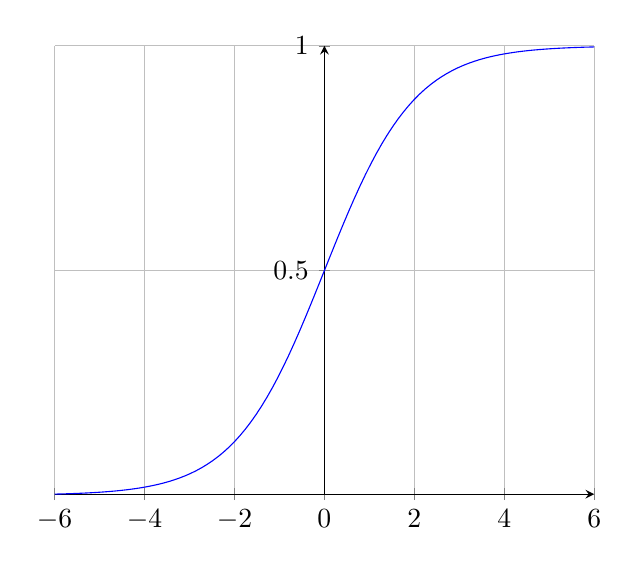
\begin{tikzpicture}
    \begin{axis}%
    [
        grid=major,     
        xmin=-6,
        xmax=6,
        axis x line=bottom,
        ytick={0,.5,1},
        ymax=1,
        axis y line=middle,
    ]
        \addplot%
        [
            blue,%
            mark=none,
            samples=100,
            domain=-6:6,
        ]
        (x,{1/(1+exp(-x))});
    \end{axis}
\end{tikzpicture}
\caption{The curve of the Sigmoid function}\label{sigmoid_curve}
\end{figure}

La régression logistique est un des modèles multivariables couramment utilisé en épidémiologie \cite{Am02,Pr05}  (c’est-à-dire l’étude de l’incidence, de la distribution et du contrôle possible des maladies et d’autres facteurs liés à des problèmes de santé pouvant affecter des groupes de population). Dans un tel contexte la variable dépendante est habituellement la survenue ou non d'un événement (maladie ou autre) et les variables indépendantes sont celles susceptibles d'influencer la survenue de cet événement c'est-à-dire les variables mesurant l'exposition à un facteur de risque ou à un facteur protecteur, ou variable représentant un facteur de confusion. L'intérêt majeur de cette technique est de quantifier la force de l'association entre chaque variable indépendante et la variable dépendante, en tenant compte de l'effet des autres variables intégrées dans le modèle \cite{Am02} .





